\documentclass{webofc}
\usepackage[varg]{txfonts}
\usepackage{graphicx}
\usepackage{minted}

% 6 pages excluding references!

\begin{document}
\title{Awkward Arrays in Python, C++, and Numba}

\author{%
\firstname{Jim} \lastname{Pivarski}\inst{1}\fnsep\thanks{\email{pivarski@princeton.edu}} \and
\firstname{Peter} \lastname{Elmer}\inst{1}\fnsep\thanks{\email{Peter.Elmer@cern.ch}} \and
\firstname{David} \lastname{Lange}\inst{1}\fnsep\thanks{\email{David.Lange@cern.ch}}}

\institute{Princeton University}

\abstract{%
  Insert your english abstract here.
}

\maketitle

\section{Introduction}

Columnar data structures, in which identically typed data fields are contiguous in memory, are a good fit to physics analysis use-cases. This was recognized as early as 1989 when column-wise ntuples were added to PAW and in 1995 when ``splitting'' was added to the ROOT file format. In the past decade, with the Google Dremel paper [ref], the Parquet file format [ref], the Arrow memory interchange format [ref], and the inclusion of ``ragged tensors'' in TensorFlow [ref], the significance of hierarchical columnar data structures has been recognized beyond particle physics.

With the exception of the Columnar Objects experiment of T.\ Mattis et.\ al.\ [ref] and the XND library [ref], all of these projects focus on representing, storing, and transmitting columnar data structures, rather than operating on them. Physicists need to apply structure-changing transformations to search for decay topology candidates and other tasks that can change the level of nesting and multiplicity of their data. Operations of this complexity can be defined as a suite of primitives, allowing for NumPy-like convenience in Python \mbox{[2018 CHEP ref].\hspace{-1 cm}}

The Awkward Array library [2018 ROOT workshop ref] was created to provide these operations on arrays that are easily convertible to the other libraries (zero-copy in some cases). Since its release in September 2018, it has become one of the most widely pip-installed packages for particle physics (see Figure~\ref{fig:pip-timeline}).

\begin{figure}
\begin{center}
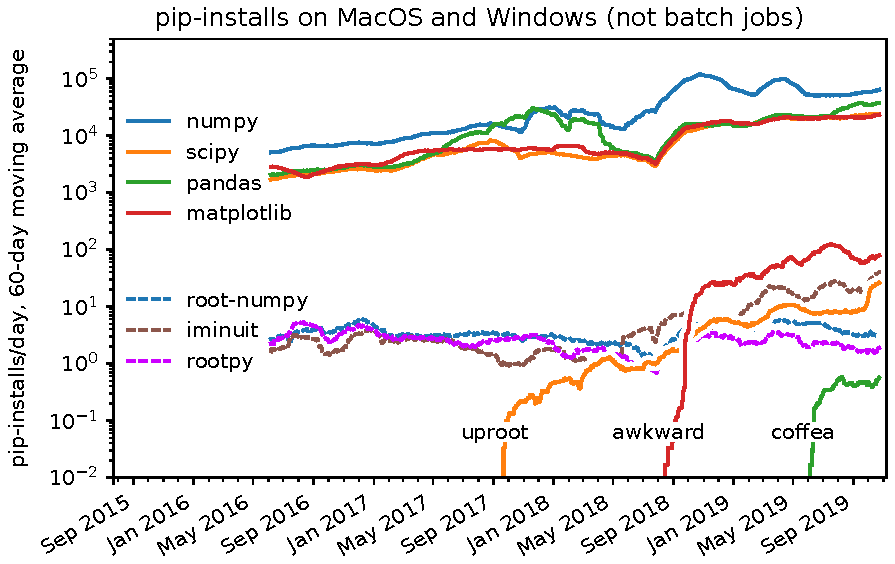
\includegraphics[width=0.7\linewidth]{pip-timeline.pdf}
\end{center}
\caption{Number of pip-installations per day (smoothed by a 60-day moving average) for popular data analysis libraries (numpy, scipy, pandas, matplotlib) and particle physics libraries (root-numpy, iminuit, rootpy, uproot, awkward, coffea) on operating systems not used for batch jobs (MacOS and Windows). \label{fig:pip-timeline}}
\end{figure}

Feedback from physicists, such as the interviews we reported previously [2019 ACAT paper ref] and in private conversations at a series of tutorials, has revealed that physicists appreciate the NumPy-like interface when it's easy to see how an analysis task can be expressed that way, but still need an interface for imperative programming. In addition, some names were poorly chosen, leading to confusion and name-conflicts, and more of the library's internal structure should be hidden from end-users. Also, the original library's pure NumPy implementation has been hard to extend and maintain.

All of these issues argue for a redesign of the library, keeping the core concepts that work, restructuring the internals for maintainance, and presenting a simpler, more uniform user interface. The Awkward Array reimplementation project has been dubbed ``Awkward 1.0'' and has been allocated as a 6-month task from September 2019 to March 2020.

\section{Architecture}

The principle of Awkward Array is that an array of any data structure can be constructed from a composition of nodes that each provide one feature. The prototypical example is a jagged array, which represents an array of unequal-length subarrays with an array of integer \mintinline{c++}{offsets} and a contiguous array of \mintinline{c++}{content}. If the \mintinline{c++}{content} is one-dimensional, the jagged array is two-dimensional, where the second dimension has unequal lengths. To make a three-dimensional jagged array (unequal lengths in both inner dimensions), one jagged array node can be used as the \mintinline{c++}{content} for another. With an appropriate set of generators, any data structure can be assembled.

In the original Awkward Array library, the nodes were Python classes with special methods that NumPy recognizes to pass array-at-a-time operations through the data structure. Although that was an easy way to get started and respond rapidly to users' needs, some tasks are more difficult to express purely in NumPy calls than others. For complete generality, Awkward 1.0 nodes are implemented as C++ classes, operated upon by specialized code.

We can satisfy users' needs for imperative access by adding Numba extensions to Awkward Array, but this would amount to rewriting the entire library, once in precompiled code (C++), and once in JIT-compiled code (Numba). To ease maintainance burdens, we have separated the Awkward 1.0 operations---specialized loops that perform array manipulations---from the persistent data structures themselves. Operations only need to be written once, and can be called from the two versions of the data structures, one in C++ and the other in Numba.

In total, there are four layers:

\begin{enumerate}
\item High-level user interface in Python, which presents a single \mintinline{python}{awkward.Array} class.
\item Nested data structure nodes: C++ classes wrapped in Python with pybind11.
\item Two versions of the data structures, one in C++ and one in Numba.
\item Awkward Array operations in specialized, precompiled code with a pure C interface (can be called from C++ and Numba).
\end{enumerate}

\noindent With one exception to be discussed in Section~\ref{lab:fillablearray}, all loops that scale with the number of entries in arrays are in layer~4. All allocation and memory ownership is in layer~3, independently implemented for C++ and Numba. This separation mimics NumPy itself, which uses Python reference counting to manage ownership and precompiled code for all operations that scale with the size of the arrays. Like NumPy/CuPy and array libraries for machine learning, we could add GPU support by reimplementing the layer~4 operations for GPU targets.

\subsection{High-level Python layer}

From a data analyst's perspective, Awkward Array is a library with one important data type, \mintinline{python}{awkward.Array}, and a suite of functions operating on that type, \mintinline{python}{awkward.*}.

\begin{minted}{python}
>>> import awkward as ak
>>> array = ak.Array([[{"x": 1, "y": [1.1]}, {"x": 2, "y": [2.0, 0.2]}],
...                   [], [{"x": 3, "y": [3.0, 0.3, 3.3]}]])
>>> array
<Array [[{x: 1, y: [1.1]}, ... 3.3]}]] type='3 * var * {"x": int64,...'>
\end{minted}

\noindent Much like NumPy's \mintinline{python}{dtype}, the actual type of the array is a Python value (expressed in DataShape [ref] notation).

\begin{minted}{python}
>>> ak.typeof(array)
3 * var * {"x": int64, "y": var * float64}
\end{minted}

\noindent These arrays can be sliced like NumPy arrays, with a mix of integers, slices, arrays of booleans and integers, jagged arrays of booleans and integers, etc.

\begin{minted}{python}
>>> array["y", [0, 2], :, 1:]
<Array [[[], [0.2]], [[0.3, 3.3]]] type='2 * var * var * float64'>
\end{minted}

\noindent They can also be operated on with NumPy's array-at-a-time functions.

\begin{minted}{python}
>>> import numpy as np
>>> np.sin(array)
<Array [[{x: 0.841, ... -0.158]}]] type='3 * var * {"x": int64,...'>
\end{minted}

The nodes that define the structure of an array, which were the basic types of the original Awkward Array library, are accessible through a \mintinline{python}{layout} property, but most physicists won't need to access this layer.

%% \begin{minted}{python}
%% >>> array.layout
%% <ListOffsetArray64>
%%   <offsets><Index64 i="[0 2 2 3]" offset="0"/></offsets>
%%   <content><RecordArray>
%%     <field index="0" key="x">
%%       <NumpyArray format="l" shape="3" data="1 2 3"/>
%%     </field>
%%     <field index="1" key="y">
%%       <ListOffsetArray64>
%%         <offsets><Index64 i="[0 1 3 6]" offset="0"/></offsets>
%%         <content>
%%           <NumpyArray format="d" shape="6" data="1.1 2 0.2 3 0.3 3.3"/>
%%         </content>
%%       </ListOffsetArray64>
%%     </field>
%%   </RecordArray></content>
%% </ListOffsetArray64>
%% \end{minted}

A surprisingly important use-case for the original Awkward Array was the ability to add domain-specific code to the data structures. For example, records with fields named \mintinline{python}{"pt"}, \mintinline{python}{"eta"}, \mintinline{python}{"phi"}, and \mintinline{python}{"mass"} were wrapped as \mintinline{python}{LorentzVector} objects, with operations on arrays of \mintinline{python}{LorentzVectors} (addition, boosting, $\Delta R$ calculations, etc.) provided as methods. However, this feature was implemented using Python class inheritance, which was fragile because new Python objects for the same data are frequently created, and it was easy to lose the necessary superclasses in these transformations.

This feature is implemented more robustly in Awkward 1.0 by only applying the interpretation when creating the high-level wrapper, and keeping track of how to interpret each \mintinline{python}{layout} node with \mintinline{python}{parameters} that pass through C++ and Numba. For example,

\begin{minted}{python}
>>> class Point(awkward1.Record):
...   def __repr__(self):
...     return "Point({} {})".format(self["x"], self["y"])
\end{minted}

\begin{minted}{python}
>>> ak.namespace["Point"] = Point
>>> array.layout.content.setparameter("__class__", "Point")
>>> array.layout.content.setparameter("__str__", "P")
>>> array
<Array [[Point(1 [1.1]), ... Point(3 [3, 0.3, 3.3])]] type='3 * var * P'>
\end{minted}

\noindent Incidentally, strings are implemented this way, too: there is no string array type, but lists of 8-bit integers that should be interpreted as strings are labeled as such, and therefore presented and operated upon as such.

\begin{minted}{python}
>>> array = ak.Array(["one", "two", "three"])
>>> ak.tolist(array)
['one', 'two', 'three']
>>> # Remove the "string" interpretation.
>>> array.layout.content.setparameter("__class__", None)
>>> ak.tolist(array)
[[111, 110, 101], [116, 119, 111], [116, 104, 114, 101, 101]]
\end{minted}

\subsection{C++ layer}

HERE

\subsection{Numba layer}

\subsection{Kernels layer}

\section{Record-oriented $\to$ columnar}
\label{lab:fillablearray}

% \subsection{Deeply nested data from ROOT}

\section{Status}

\section{Conclusion}




%% \section{Introduction}
%% \label{intro}
%% Your text comes here. Separate text sections with

%% \section{Section title}
%% \label{sec-1}
%% For bibliography use \cite{RefJ}

%% % BibTeX or Biber users please use (the style is already called in the class, ensure that the "woc.bst" style is in your local directory)
%% % \bibliography{name or your bibliography database}
%% %
%% % Non-BibTeX users please use
%% \begin{thebibliography}{}
%% % and use \bibitem to create references.
%% \bibitem{RefJ}
%% Journal Author, Journal \textbf{Volume}, page numbers (year)
%% \end{thebibliography}

\end{document}
